% プロジェクト学習中間報告書書式テンプレート ver.1.0 (utf-8)

% 両面印刷する場合は `openany' を削除する
\documentclass[openany,11pt,papersize,dvipdfm]{jsbook}

%\usepackage[final]{funpro}%最終報告書
\usepackage[middle]{funpro}%中間報告書

\usepackage{graphicx}

\def\hissu{\bgroup\color{red}}
\def\endhissu{\egroup}

\thisYear{2023}

\jProjectName{使ってもらって学ぶフィールド指向システムデザイン 2023}

\eProjectName{Field Oriented System Design Learning by Users' Feedback 2023}

\ProjectNumber{3-A}

\jGroupName{グループ A}
\eGroupName{Group~A}

\ProjectLeader{佐々木虎太郎}{Kotaro~Sasaki}

\GroupLeader  {及川寛太}{Kanta~Oikawa}
\SumOfMembers{5}
\GroupMember {1}{及川寛太}{Kanta~Oikawa}
\GroupMember {2}{下村蒔里萌}{Marimo~Shimomura}
\GroupMember {3}{大津武琉}{Takeru~Otsu}
\GroupMember {4}{稲田敬介}{Keisuke~Inada}
\GroupMember {5}{ディオガーディディラン基暉}{Dylan~Motoki~Dioguardi}

\jadvisor{伊藤恵,南部美砂子,奥野拓,元木環,石尾隆}
\eadvisor{Kei~Ito,Misako~Nambu,Taku~Okuno,Tamaki~Motoki,Takashi~Ishio}

\jdate{2023年7月21日}
\edate{July~21, 2023}

\begin{document}

\maketitle

\frontmatter

\begin{jabstract}
 本プロジェクトは,フィールド調査をもとにした活動で発見した問題を,IT を用いて解決する.これは,ユーザの仕事や生活をデザインし,地域や社会に貢献することが目的である.本プロジェクトでは,アジャイル開発手法を用いる.迅速で柔軟な開発を行い,短期間の開発で効果的な成果を出すことが目的である.15名のメンバーが「交通」「小学校支援」「未来大生支援」のフィールドで活動する. 本報告では交通グループについての報告を行う.

 本グループでは,ブレインストーミングを行った中で発見したバスの使いにくいという問題を解決することを目的として活動している.具体的には,いつバス停に行けばいいのかがわからない, 乗りたいバスに間に合うかどうかがわからないという問題が存在する.既存のバスロケーションアプリは,情報量が多く,この問題を解決できていなかった.また,バスの現在の正確な位置や,バス停への発着情報がわかりにくいという問題があった.そこで,情報量が絞られており,一目でバスと自分の位置関係がわかるアプリの開発を検討している.これまで,見やすいUI,洗練された機能についての考察,開発を行ってきた.今後は,引き続き開発を進め,早期リリースを目指しながら取り組んでいく.
\begin{jkeyword}
バス,遅延,情報量過多,交通,モバイルアプリ,ひとめぼれ,デザイン,体験,アジャイル,スクラム,フィールド調査,函館
\end{jkeyword}
\bunseki{大津武琉}
\end{jabstract}

\begin{eabstract}
This project aims to solve the problems found in field research using IT. This is to design the user's work and life, and contribute to the community and society. This project uses an agile development method. The purpose is to quickly and flexibly develop and achieve effective results in a short period of development. 15 members work in the fields of "transportation", "elementary school support", and "FUN students support". This report reports on the transportation group.

The group aims to solve the problem of inefficient use of buses found through brainstorming. Specifically, there is the problem of not knowing when to go to the bus stop and whether you will be able to catch the bus you want. Existing bus location apps have a lot of information and have not been able to solve this problem. In addition, the current accurate position of the bus and the departure and arrival information to the bus stop are difficult to understand. Therefore, we are considering developing an app that has a limited amount of information and can see the bus and your position relationship at a glance. So far, we have been thinking about and developing a user interface that is easy to see and refined functions. In the future, we will continue to develop and strive for early release.
\begin{ekeyword}
Bus, Delay, Information Overload, Transportation, Mobile App, Fall in Love at First Glance/Use, Design, Experience, Agile, Scrum, Field Research, Hakodate
\end{ekeyword}
\bunseki{大津武琉}
\end{eabstract}

\tableofcontents

\mainmatter

\chapter{はじめに}

\section{プロジェクトの立ち上げ}
世の中にはニーズを十分に満たしていないシステムが存在する.これは,開発者が作るものとユーザが求めるものとの乖離が原因の1つであると考えられる.この問題を解決するためには,ユーザを理解してシステムを開発する必要があることから,開発者が現場に赴き,調査をして,ユーザから直接学ぶべきであると考えた.そこで「使ってもらって学ぶフィールド指向システムデザイン」を理念とするプロジェクトが始まった.
\bunseki{稲田敬介}

\section{プロジェクトの方針}
本プロジェクトは,例年実際に現場に赴くフィールド調査とアジャイル開発手法の 1 つである,スクラム手法 \cite{scrum}を採用している.フィールド調査ではユーザの思考や行動などの,現場に行かないと分からないことを知ることができる.また,スクラムは,アジャイル開発の中でも少人数のチームで開発を行い,スプリントと呼ばれる固定の短い時間に区切って作業を進めるものである\cite{scrum}.これはユーザのフィードバックを繰り返し受けて,改善する機会を何度も得ることができるため,本プロジェクトの「使ってもらって学ぶフィールド指向システムデザイン」という理念と合致する.以上のことから,今年度もフィールド調査とスクラム手法を採用することにした.
\bunseki{ディオガーディディラン基暉}

\section{交通グループ}\label{sec:gaiyou}
発車予定時刻ギリギリにバス停についたときに,バスが今どこにいるのかがわからないことで, バスがもう行ってしまったのか, まだ来ていないのかがわからないという現状がある.また,現在存在する地図アプリや,乗換案内のアプリ,バス会社が提供しているバスロケーションシステムによって,バスの運行に関する情報を手に入れることができる.しかし,それらの情報は大量で整理されておらず, 欲しい情報に辿り着くのが難しい.先述の問題を既存のアプリやシステムで解決することが困難であることから,本グループでは,バス利用者がストレスを抱えずにバスを利用できるようなアプリ開発を行うことにした.
\bunseki{大津武琉}

\chapter{中間発表までの主な活動}

\section{ブレインストーミング}
まず各々がこのチームで開発したいアイディアを,Miro\footnote{https://miro.com/}を使用して,書き出した.アイディアの例は以下である.

\begin{quote}
    \begin{itemize}
        \item 独り言を自動的に録音してテキスト化
        \item 健康促進アプリ(地図上でこれまで行った場所を塗りつぶす)
        \item 悩みがある人同士で会話できるもの
        \item 店など様々な場所の混雑度チェックアプリ
        \item 公共交通機関を携帯からリアルタイムに把握する
        \item 1日を可視化
    \end{itemize}
\end{quote}

各々違う色の付箋を使用し,KJ法を使用し意見をまとめた.この活動ではさまざまな意見が挙げられたが,一番チームの共感を得たバスについて,今後の活動を絞った.

\begin{figure}[htbp]
    \centering
    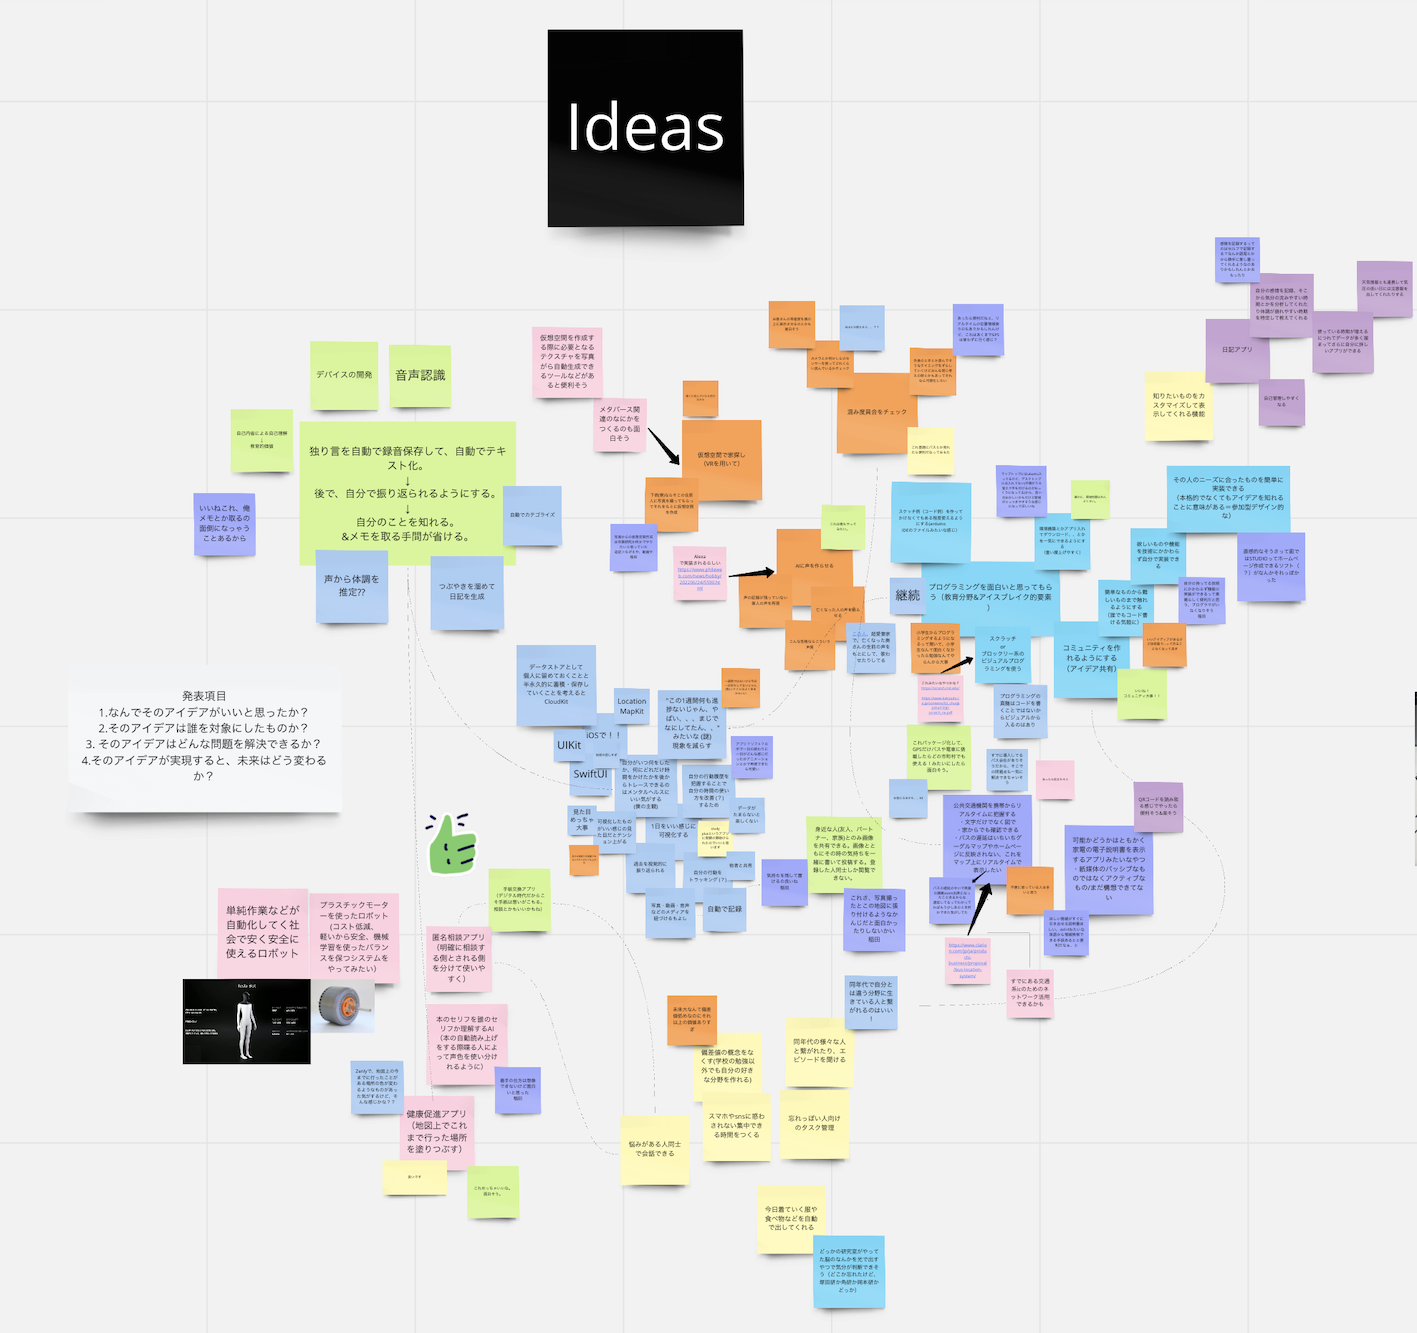
\includegraphics[width=9cm]{images/brainstorm.png}
    \caption{ブレインストーミング}
    \label{fig:brainstorm}
\end{figure}
\bunseki{大津武琉}

\section{アイディアの深掘り}

上記のブレインストーミングで挙げられたアイディアは煩雑なものであったため,実際に我々がバスを利用してきた中で不便に感じたことを考え,欲しい機能を列挙していった.機能の例は以下である.

\begin{quote}
    \begin{itemize}
        \item 交通系ICカードを取り込み残高を表示
        \item バス停までの徒歩時間表示
        \item バスの時刻表表示
        \item 地図上に表示するバスの数を変えれる
    \end{itemize}
\end{quote}

\begin{figure}[htbp]
    \centering
    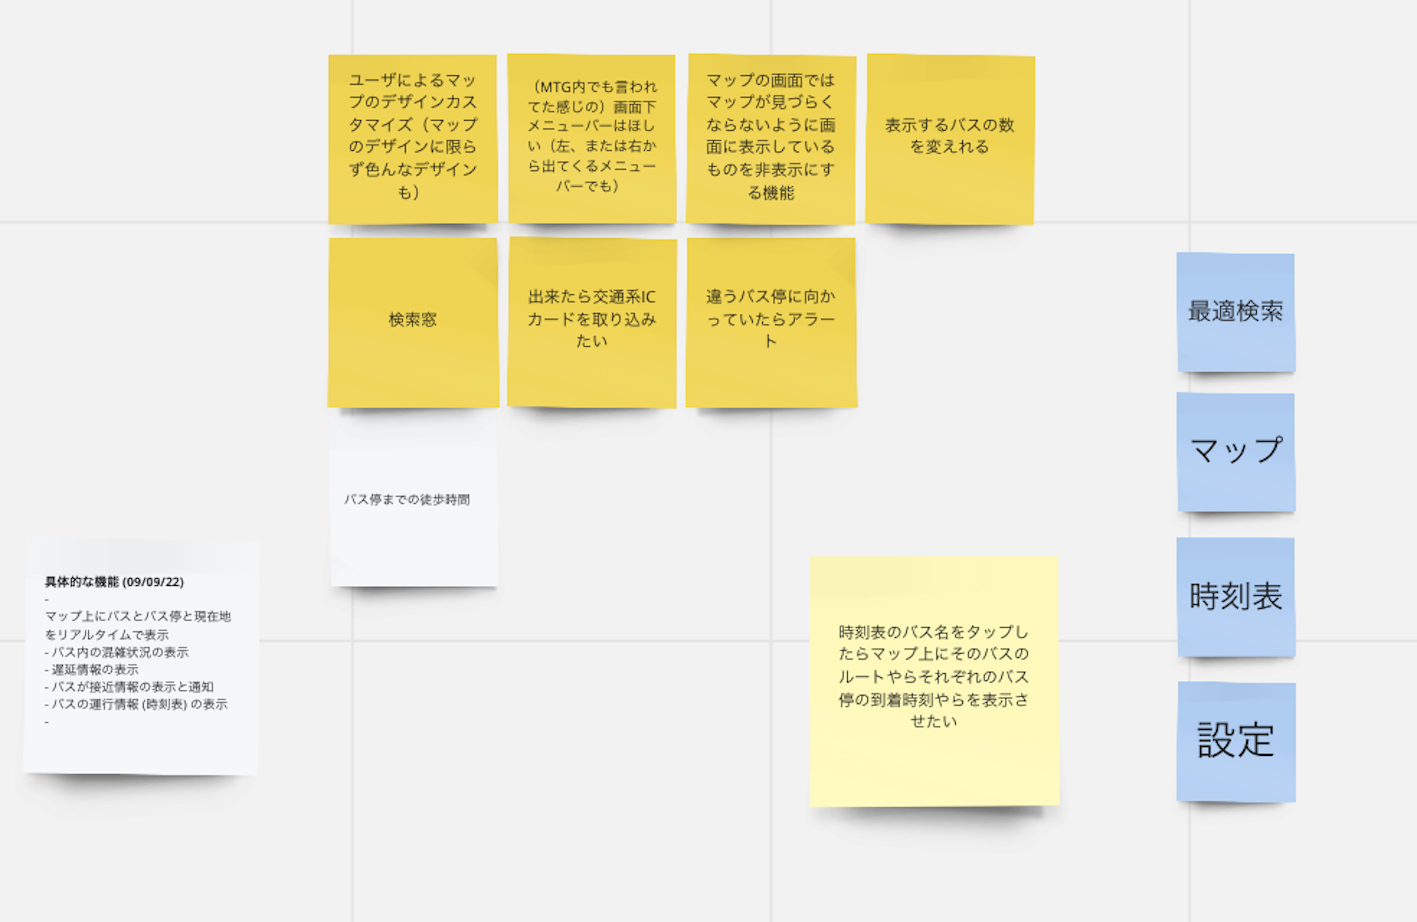
\includegraphics[width=9cm]{images/dig.png}
    \caption{アイディアの深掘り}
    \label{fig:dig}
\end{figure}
\bunseki{下村蒔里萌}


\section{開発プラットフォームの決定}
まず,iOSとAndroidの2プラットフォームのネイティブアプリを並行して開発するか,クロスプラットフォームのネイティブアプリを開発するか,ということについて考えた.本グループでは2つの理由からクロスプラットフォーム開発に決定した.1つ目の理由は,グループの規模が小さいことである.プラットフォームを分けると,各プラットフォーム2〜3人となってしまい各人の負担が大きい.2つ目の理由は,本グループ全体の技術力が少ないことである.本グループには,過去に開発者としてアプリケーション開発を行ったことのある者が1人しかいない.ほかのメンバーは経験がなく,1から学習を始めるため,学習コストが大きい.以上の理由より,クロスプラットフォームのネイティブアプリの開発を進める形となった.使用するフレームワークはクロスプラットフォームの代表例であるFlutter\footnote{https://flutter.dev/}となった.
\bunseki{及川寛太}

\section{メンバーの役割決定}
本グループでは5人のメンバーで行っている.各メンバーの役割については以下の通りとなっている.

\subsection{プロダクトオーナー}
プロダクトオーナーはプロダクトの責任者であり,開発チームを活用して,そのプロダクトが生み出す価値を最大化する責任がある\cite{scrum}.
\begin{quote}
    \begin{itemize}
        \item 及川 寛太
    \end{itemize}
\end{quote}

\subsection{スクラムマスター}
スクラム開発を円滑に進める役割がある.具体的に,アジャイルとスクラムの価値を維持し,ほかの人がスクラムを理解し実践するのを助ける,スクラムのミーティングをファシリテートする \cite{scrummaster}.
\begin{quote}
    \begin{itemize}
        \item 大津 武琉
    \end{itemize}
\end{quote}

\subsection{デザイン}
問題やユーザ像の分析より,アプリのUXやUIを考え,Figma\footnote{https://www.figma.com/}でプロトタイプを作成する.実際にプログラムを書く際に必要な,レスポンシブな数値などのデザインシステムを作成する.
\begin{quote}
    \begin{itemize}
        \item 下村 蒔里萌
    \end{itemize}
\end{quote}

\subsection{iOSアプリ}
クロスプラットフォーム開発を行うが,iOS独自の開発が必要な場合や問題が発生した場合に,優先多岐に対応にあたる.
\begin{quote}
    \begin{itemize}
        \item 及川 寛太
        \item 下村 蒔里萌
    \end{itemize}
\end{quote}
\pagebreak
\subsection{Androidアプリ}
クロスプラットフォーム開発を行うが,Android独自の開発が必要な場合や問題が発生した場合に,優先多岐に対応にあたる.
\begin{quote}
    \begin{itemize}
        \item 大津 武琉
        \item 稲田敬介
        \item ディオガーディディラン基暉
    \end{itemize}
\end{quote}

\subsection{サーバ}
バスの運行に関わるデータの収集・記録・管理を行う.また,クライアント側が必要とする情報を素早く提供するシステムを開発する.
\begin{quote}
    \begin{itemize}
        \item 及川 寛太
        \item 大津 武琉
    \end{itemize}
\end{quote}
\bunseki{大津武琉}

\section{Git・GitHubの習得}
チーム開発を進める中で必要不可欠であるバージョン管理アプリのGitHub\footnote{https://github.com/}の勉強会を行なった.メンバーの過半数がGitHubを触ったことがなかったため,使用経験がある人から基本的な使用方法を教えてもらい,実際にGit\footnote{https://git-scm.com/}の機能であるClone,Commit,Push,Fetch,Merge,Pullを行なってGitHubについて学んだ.
\bunseki{ディオガーディディラン基暉}

\section{アプリ名の決定}
アプリの名前を考えることで,開発を進める上でのモチベーション維持を目指した.各々アプリ名を1つ以上考えることとなり以下のようなアプリ名が挙げられた.

\begin{quote}
    \begin{itemize}
        \item BuLo (ブーロ) : BusとLocationの頭をとったもので,美しく (Beautiful) ,有用なユーザーインターフェースUseful (UserInterface) を持つライブ (Live) で最良のオプション (Option) である.バスロケーションシステムという意味も持つ.
        \item Loco (ロコ) :「ロケーション」と「どこ」をかけたもの.
        \item nnuts (ナッツ) : No trouble with busの各単語から1文字とって組み合わせたもの.
        \item バスらく: バスをらくに使えるアプリを略したもの.横文字のアプリ名がたくさんあるが,ぱっと思い出しにくいため,名前からすぐにどんな用途かわかるものを提案した.
        \item ばすけん: バス検索を省略したもの.
    \end{itemize}
\end{quote}

上記のものでメンバー内で多数決をとった結果,BuLo (ブーロ) という名前に決定した.

\begin{figure}[htbp]
    \centering
    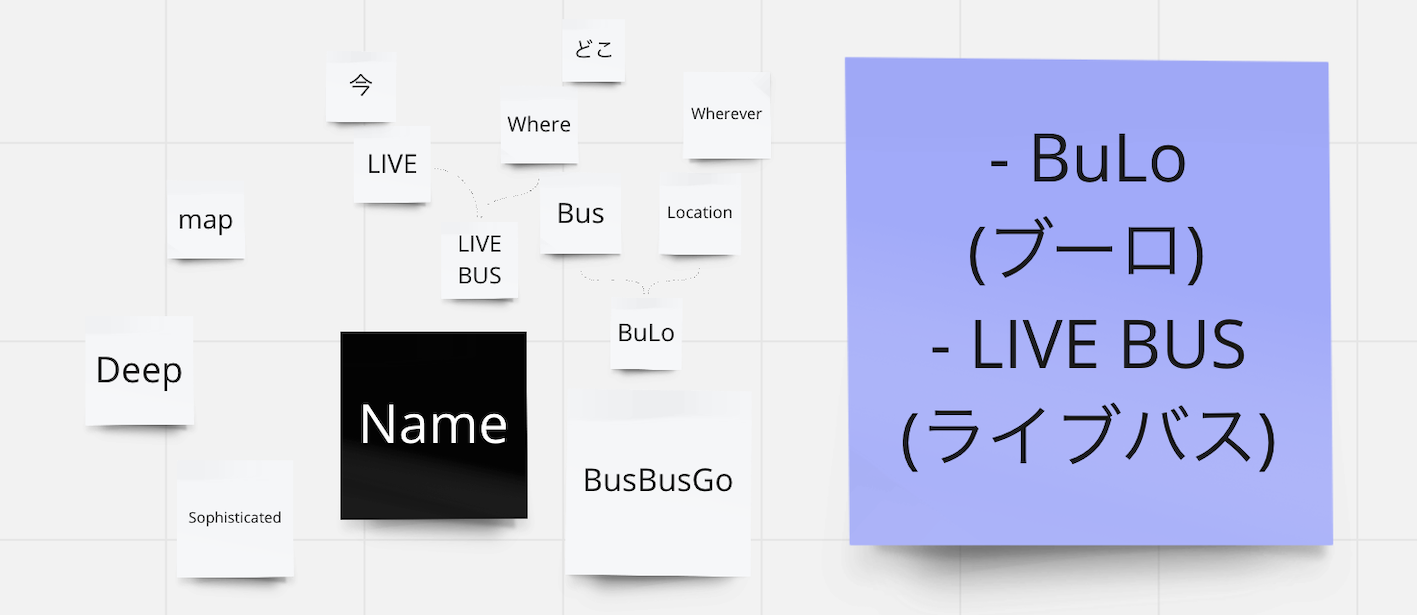
\includegraphics[width=9cm]{images/app_name.png}
    \caption{アプリ名案}
    \label{fig:app_name}
\end{figure}
\bunseki{稲田敬介}


\section{プロトタイプの作成}
イメージするアプリのプロトタイプをFigma\footnote{https://www.figma.com/}を用いて作成した (図2.4) .左から1枚目の画面は自分の現在地を表示させている.2〜4枚目は目的地を入力する画面となっている.5〜6枚目は現在地から2〜3枚目で入力した場所までのバスを表示させる.7枚目では5〜6枚目で選択したバスと自分との位置関係をグラフと地図で表示させる.

\begin{figure}[htbp]
    \centering
    \includegraphics[width=12cm]{images/prototype_v2.png}
    \caption{プロトタイプ}
    \label{fig:prototype_v2}
\end{figure}

\subsection{フィードバック}
実際にプロジェクトメンバーにFigma\footnote{https://www.figma.com/}で作成した図2.4のプロトタイプを使用してもらった.その際たくさんの質問,指摘,意見をいただいた.一番右の画面に対して,「下のバスと人との位置関係のグラフはいるのか?」,「現在動いているバスの位置情報と自分の位置情報が分かれば大体どれくらいにバス停にいけばいいのかわかるのでは?」という意見をいただいた.それらの意見に対し,ターゲットユーザを絞ることとした.

\subsection{ターゲットユーザ}
実際に得たフィードバックから,ターゲットユーザがしっかりと定まっておらず,このアプリは何のため,誰のためのアプリなのかがわからないことに気がついた.そこでチームでもう一度ターゲットユーザについて話し合い以下のように確立させた.

\begin{quote}
    \begin{itemize}
        \item 通勤通学にバスを使っていて,バスの乗降地点が毎回同じ
        \item バスに乗り遅れたくない
        \item バス停で待ちたくない
        \item 10代後半から20代前半
    \end{itemize}
\end{quote}

\subsection{改善}
確立させたターゲットユーザに合う機能のみを実装するとしたため,合わせてプロトタイプを改善した.

図2.4のプロトタイプではユーザが毎回移動先・移動元を検索していたが,最初に登録をすることで,検索を毎回行う工程を省いた.通勤通学など,使用するバスが決まっているというユーザ像には,地点の検索は無駄な工程であった.

アプリ全体のデザインとしては,色やアイコンを改善した.具体的には,Time-Distace Viewのアイコンとその色を変更した.以前は人のアイコンが走っている人間のアイコンであり,赤色を使用していたため,焦りを与えていた.そのため,色を改善し,さらに同レベルの情報の色のコントラストを揃えた.また,Flutter\footnote{https://flutter.dev/}で開発をするにおいて,アイコンをmaterial designに統一した.

また,Time-Distance Viewについて,どの駅を使用するのか,何円かかるか,何時に到着するかなどの,ユーザが必要最低限と感じる情報を追加した.また,ウィジェット全体のサイズやレイアウトを改善した.

最後に,アプリを開いた時にランディング画面を設けることで,アプリ全体の概要や印象をユーザがわかりやすくなるよう改善した.

\begin{figure}[htbp]
    \centering
    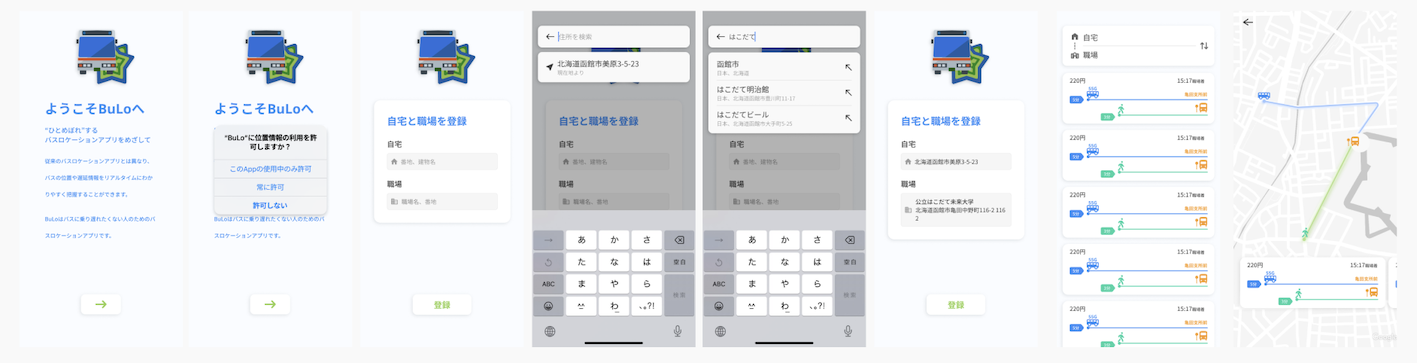
\includegraphics[width=12cm]{images/prototype_v3.png}
    \caption{フィードバックをもとに改善したプロトタイプ}
    \label{fig:prototype_v3}
\end{figure}
\bunseki{下村蒔里萌}

\section{函館バス株式会社への訪問}
函館バス株式会社は,バス運行に関するデータを公開していないため,本グループが開発しているアプリの紹介と,データを使用させていただくために,6月16日 (金) に本グループメンバーと担当教員で函館バス株式会社に訪問した.そこで函館バス株式会社の方から「新しい観点からの機能でいい」というお言葉をいただき,データの使用の許可をいただいた.

\begin{figure}[htbp]
    \centering
    \includegraphics[width=9cm]{images/hakodate_bus.png}
    \caption{函館バス株式会社訪問時の様子}
    \label{fig:hakodate_bus}
\end{figure}
\bunseki{大津武琉}

\section{中間発表}
\subsection{中間発表資料の作成}
7月7日に行われる中間発表会に向けてスライド,メインポスター (図2.7) ,サブポスター (図2.8) を作成した.これらの資料に関して教員に繰り返しレビューをしていただき,より伝わりやすいものへと改良を重ねた.

\begin{figure}[htbp]
    \centering
    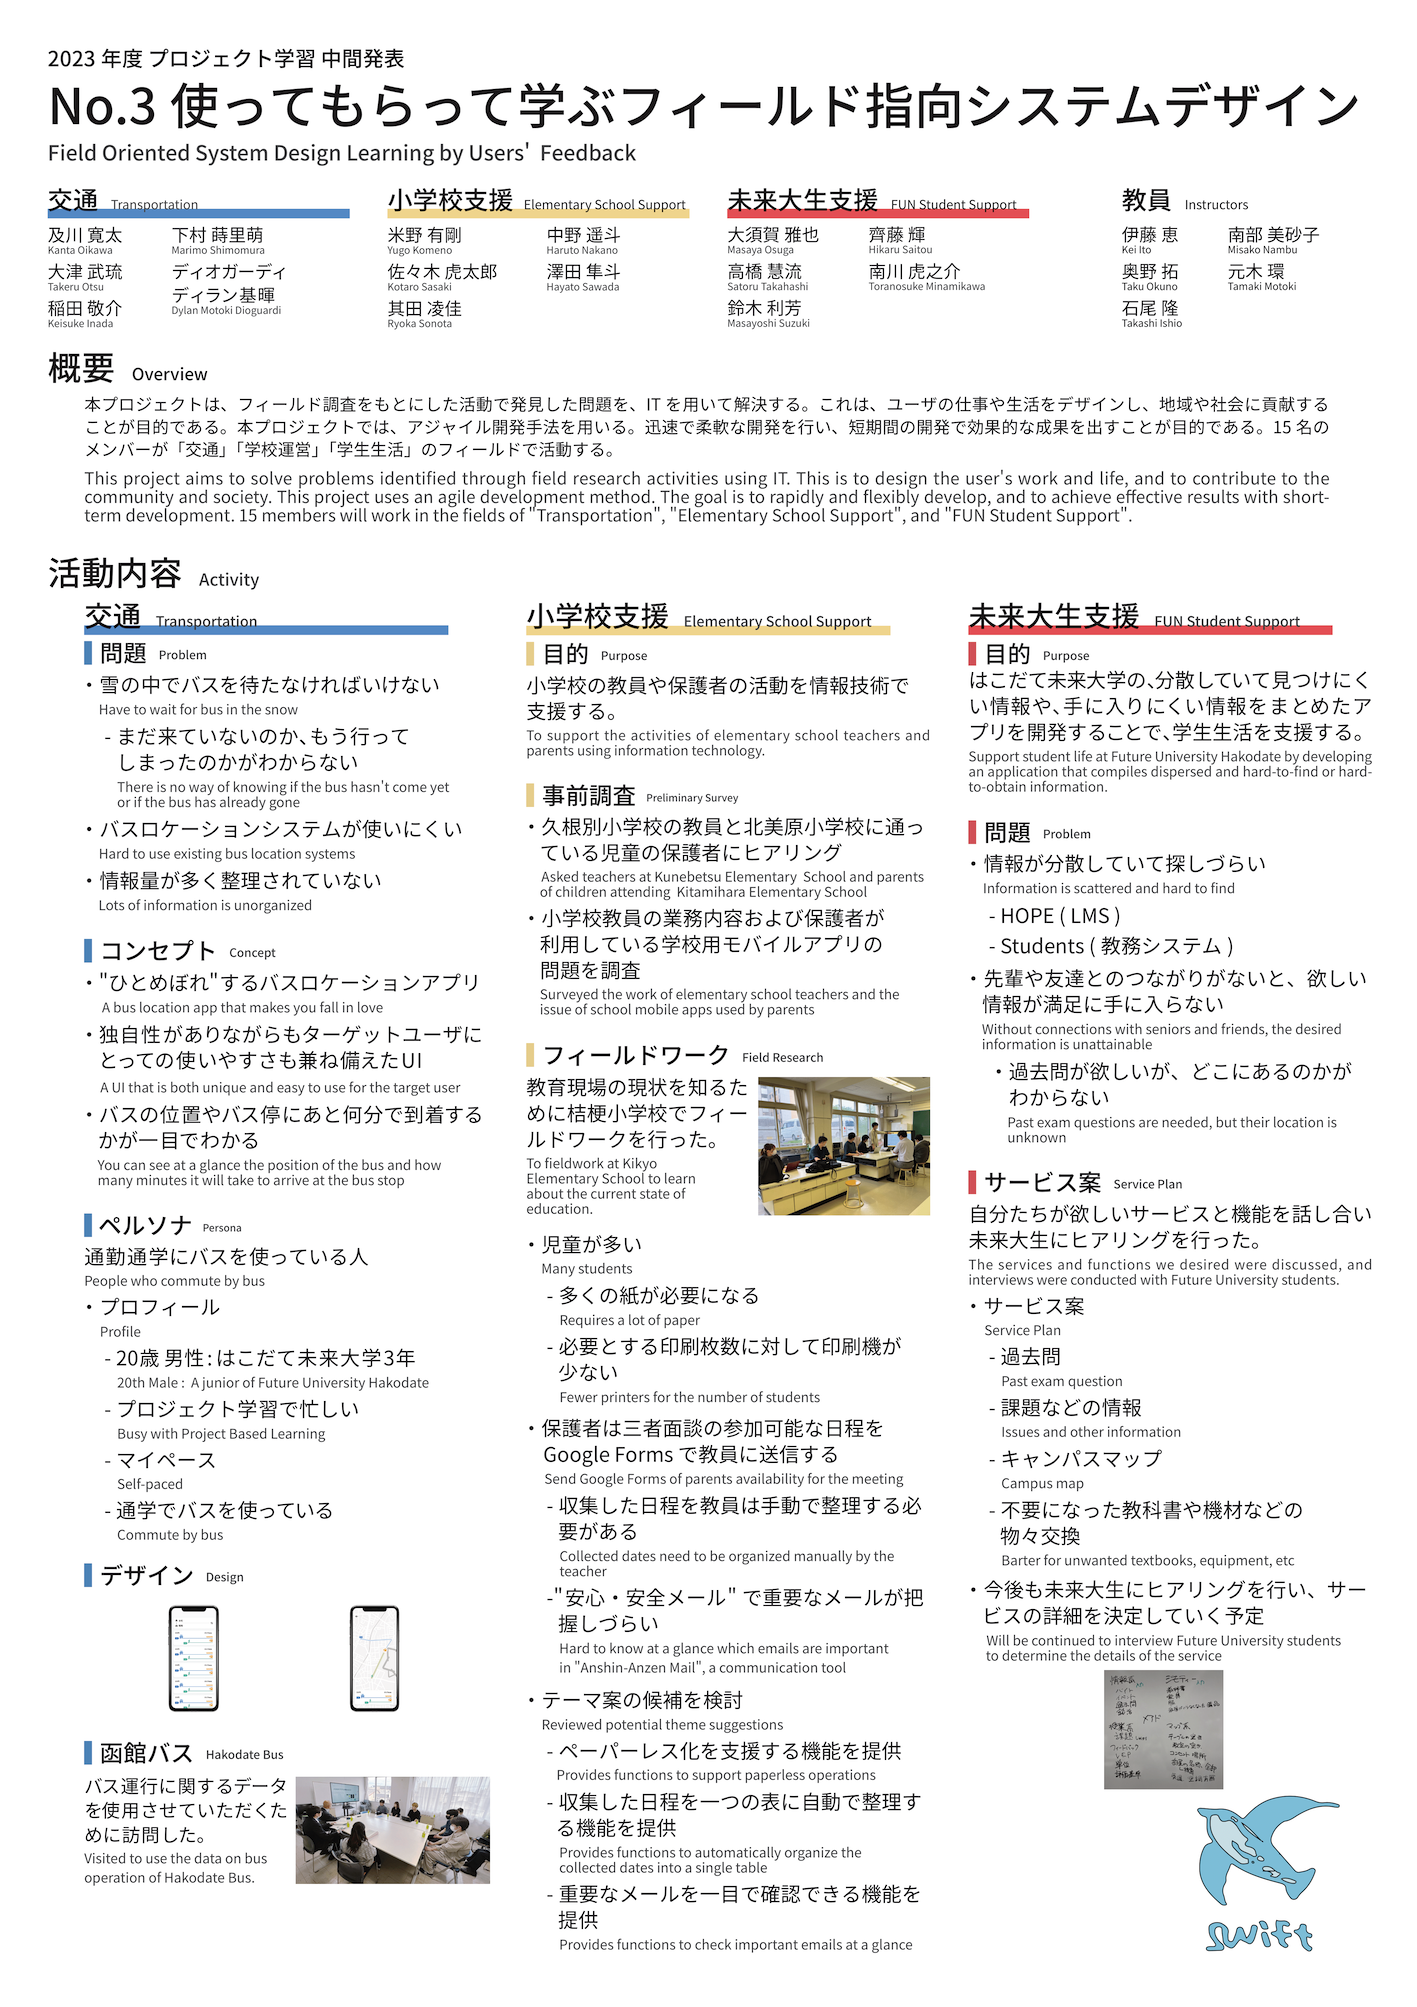
\includegraphics[width=9cm]{images/interim_poster.png}
    \caption{中間発表会メインポスター}
    \label{fig:feature_timedistanceview}
\end{figure}

\begin{figure}[htbp]
    \centering
    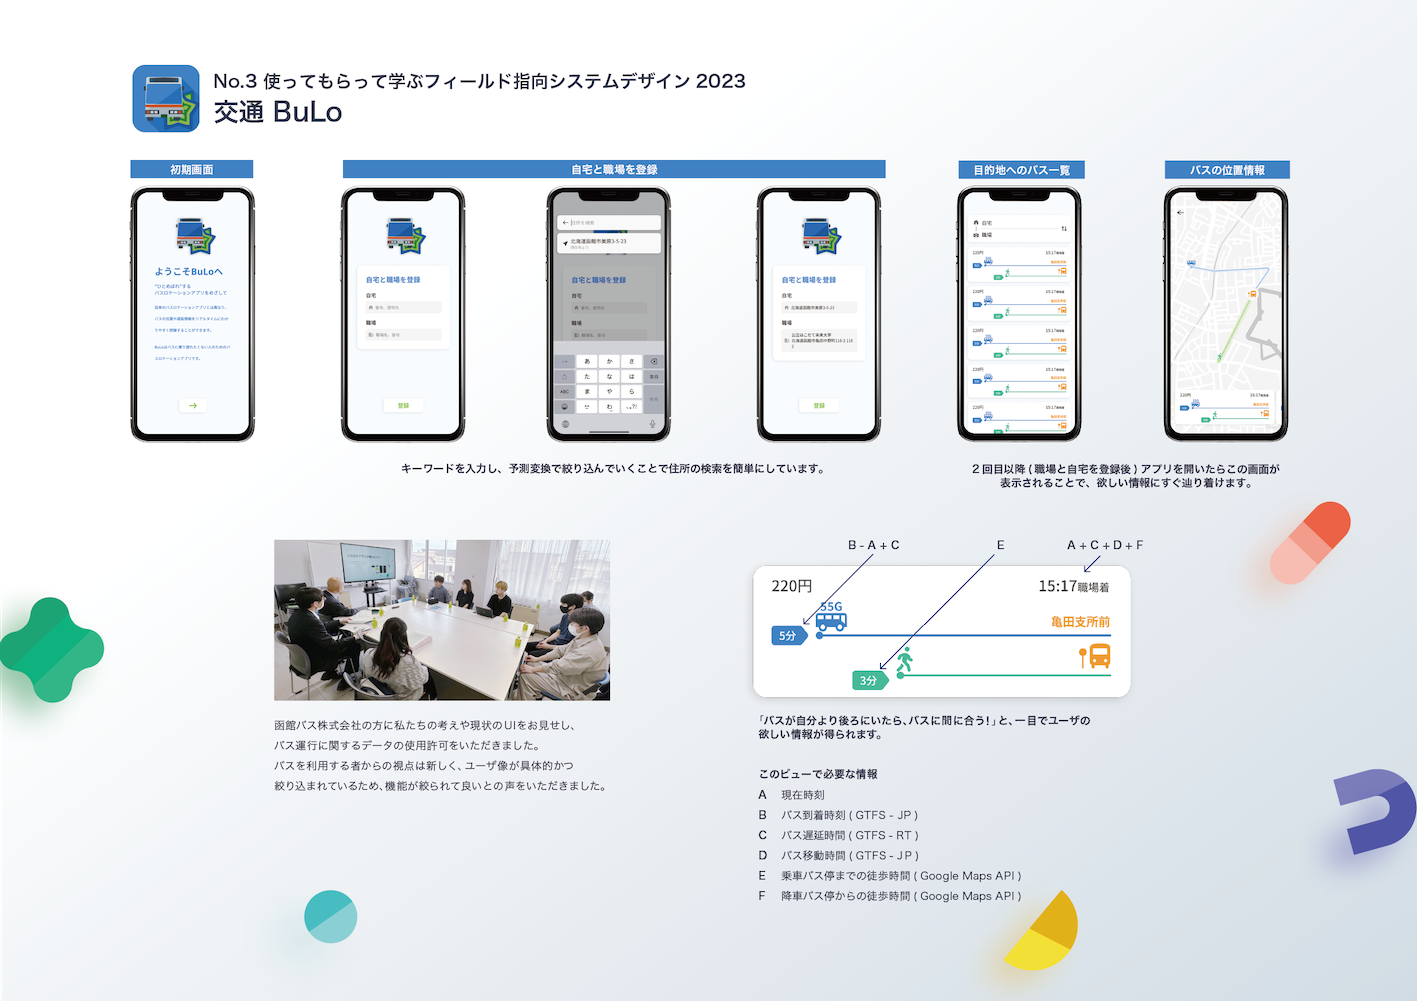
\includegraphics[width=9cm]{images/interim_poster_bulo.png}
    \caption{中間発表会サブポスター}
    \label{fig:interim_poster_bulo}
\end{figure}
\pagebreak
\subsection{中間発表会}
7月7日 (金) に発表会は行われた.そこで様々な質問や意見をいただいた.「首都圏と函館で同じ状況を想定していいのか?」「独自性を掲げているがUIについての独自性のみで機能についての独自性がみられない」という指摘をいただいた.これらの意見は,ターゲットユーザを絞り,合わせて実装する機能を絞った結果であると考えているため,次期バージョンにていただいた指摘をもとに改善を行う.

\begin{figure}[htbp]
    \centering
    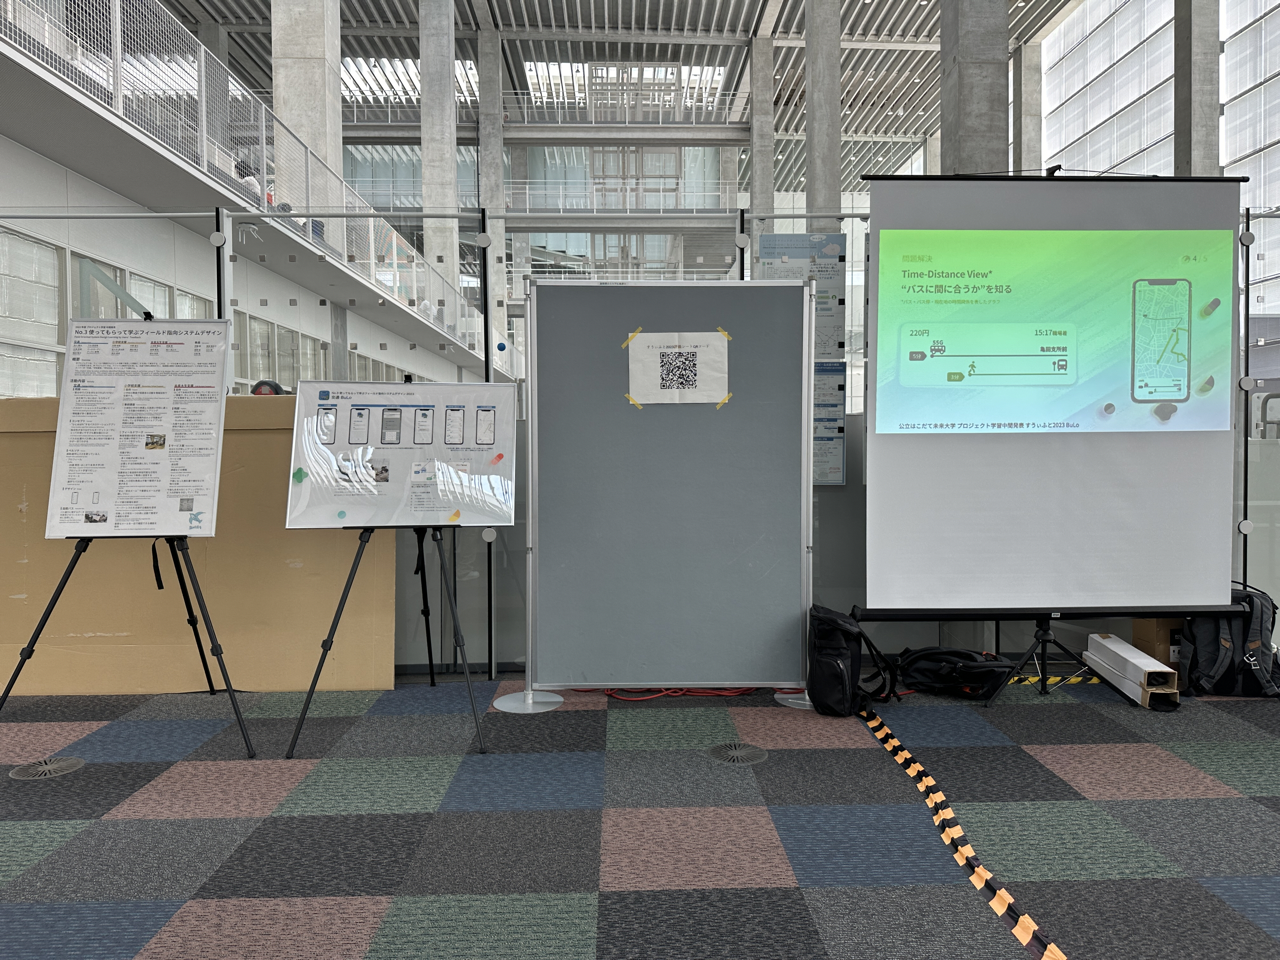
\includegraphics[width=12cm]{images/mid_presentation.png}
    \caption{中間発表会の様子}
    \label{fig:mid_presentation}
\end{figure}
\bunseki{下村蒔里萌}

\chapter{アプリケーションのアイディア}

\section{コンセプト}
BuLoはバスに乗り遅れたくないひとのためのバスロケーションアプリである.従来のバスロケーションアプリやGoogle Mapsなどの地図アプリとは異なり,バスの位置や遅延情報をリアルタイムにわかりやすく把握することができる.また,“ひとめぼれ”するバスロケーションアプリをめざしている.本グループは”ひとめぼれ”を以下の2つと考える.まず1つ目にアプリのデザインに対する”ひとめぼれ”である.これはアプリを使うきっかけとなるものである.2つ目にアプリ全体を通しての体験への”ひとめぼれ”である.これは,アプリを使い続けるきっかけになると考える.
\bunseki{及川寛太}

\section{機能}
\subsection{住所を登録}
このアプリの対象ユーザは通勤・通学にバスを利用する人であるため,自宅と職場の住所を登録する機能を搭載する.対象ユーザの使用するルートは変わらないため,最初に登録することで,2回目以降は検索をする手間を省いている.図中の左から2枚目の画面では現在地の住所を表示させている.左から3枚目の画面では「はこだて」と入力して,それに対しての予測を表示させている.

\begin{figure}[htbp]
    \centering
    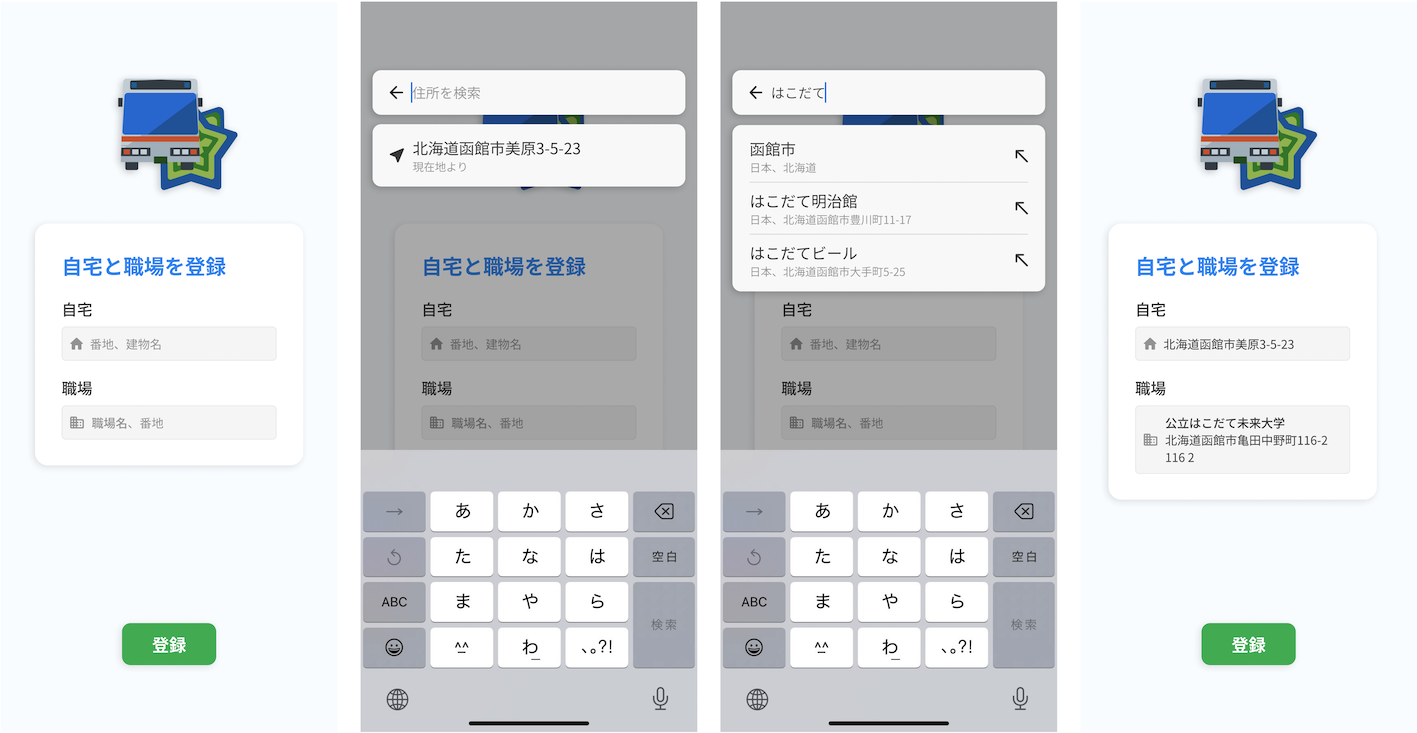
\includegraphics[width=12cm]{images/feature_registration.png}
    \caption{住所登録機能}
    \label{fig:feature_registration}
\end{figure}
\pagebreak
\subsection{Time-Distance View}
これは人とバス,バス停の距離を時間的グラフに表すことでパッとみてユーザとバスの位置関係を把握することができる.実装方法は図\ref{fig:feature_timedistanceview}に示す.図\ref{fig:feature_timedistanceview}では以下の状況を考えている.

\begin{quote}
    \begin{itemize}
        \item 目的地は職場
        \item 現在地からの最寄りのバス停は亀田支所前
        \item 乗るバスは55G
        \item 最寄りバス停から目的地付近のバス停までの料金は220円
        \item バスが5分後に亀田支所前に到着
        \item 亀田支所前まで歩きで3分
    \end{itemize}
\end{quote}

\begin{figure}[htbp]
    \centering
    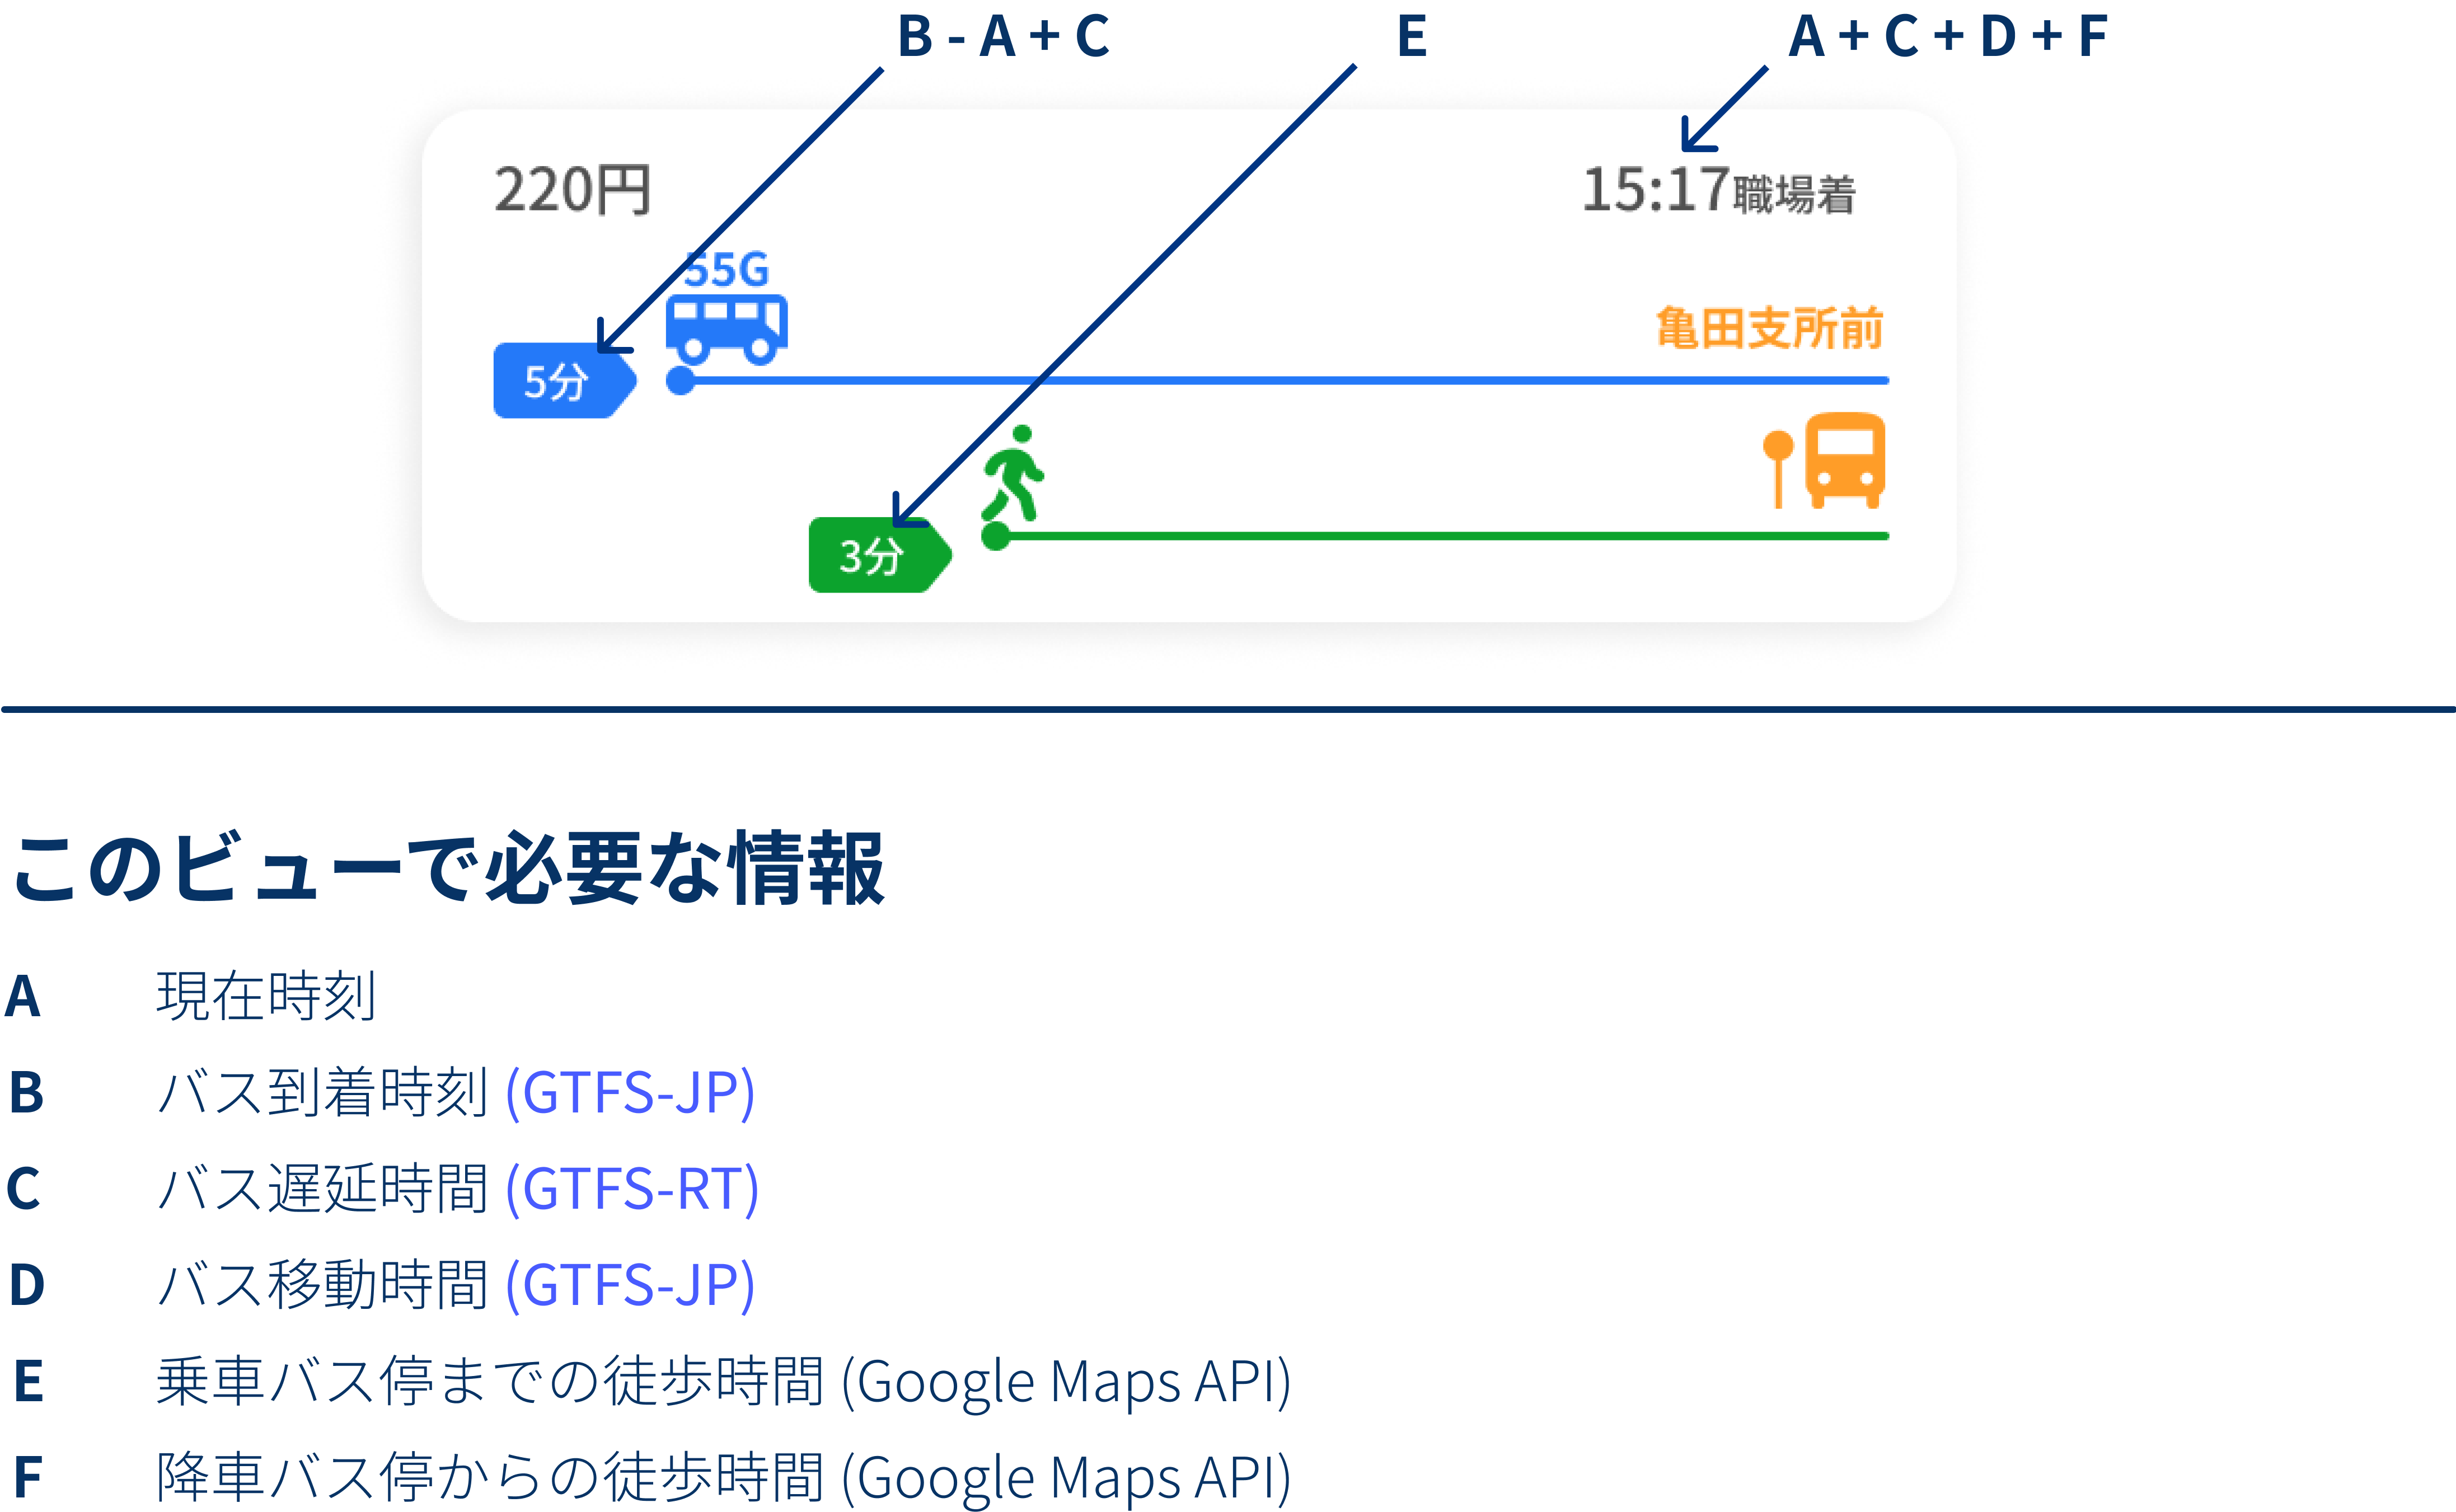
\includegraphics[width=12cm]{images/feature_timedistanceview.png}
    \caption{Time-Distance View}
    \label{fig:feature_timedistanceview}
\end{figure}
\pagebreak
\subsection{バスの位置情報}
地図上でバスとユーザの位置を確認することができる.

\begin{figure}[htbp]
    \centering
    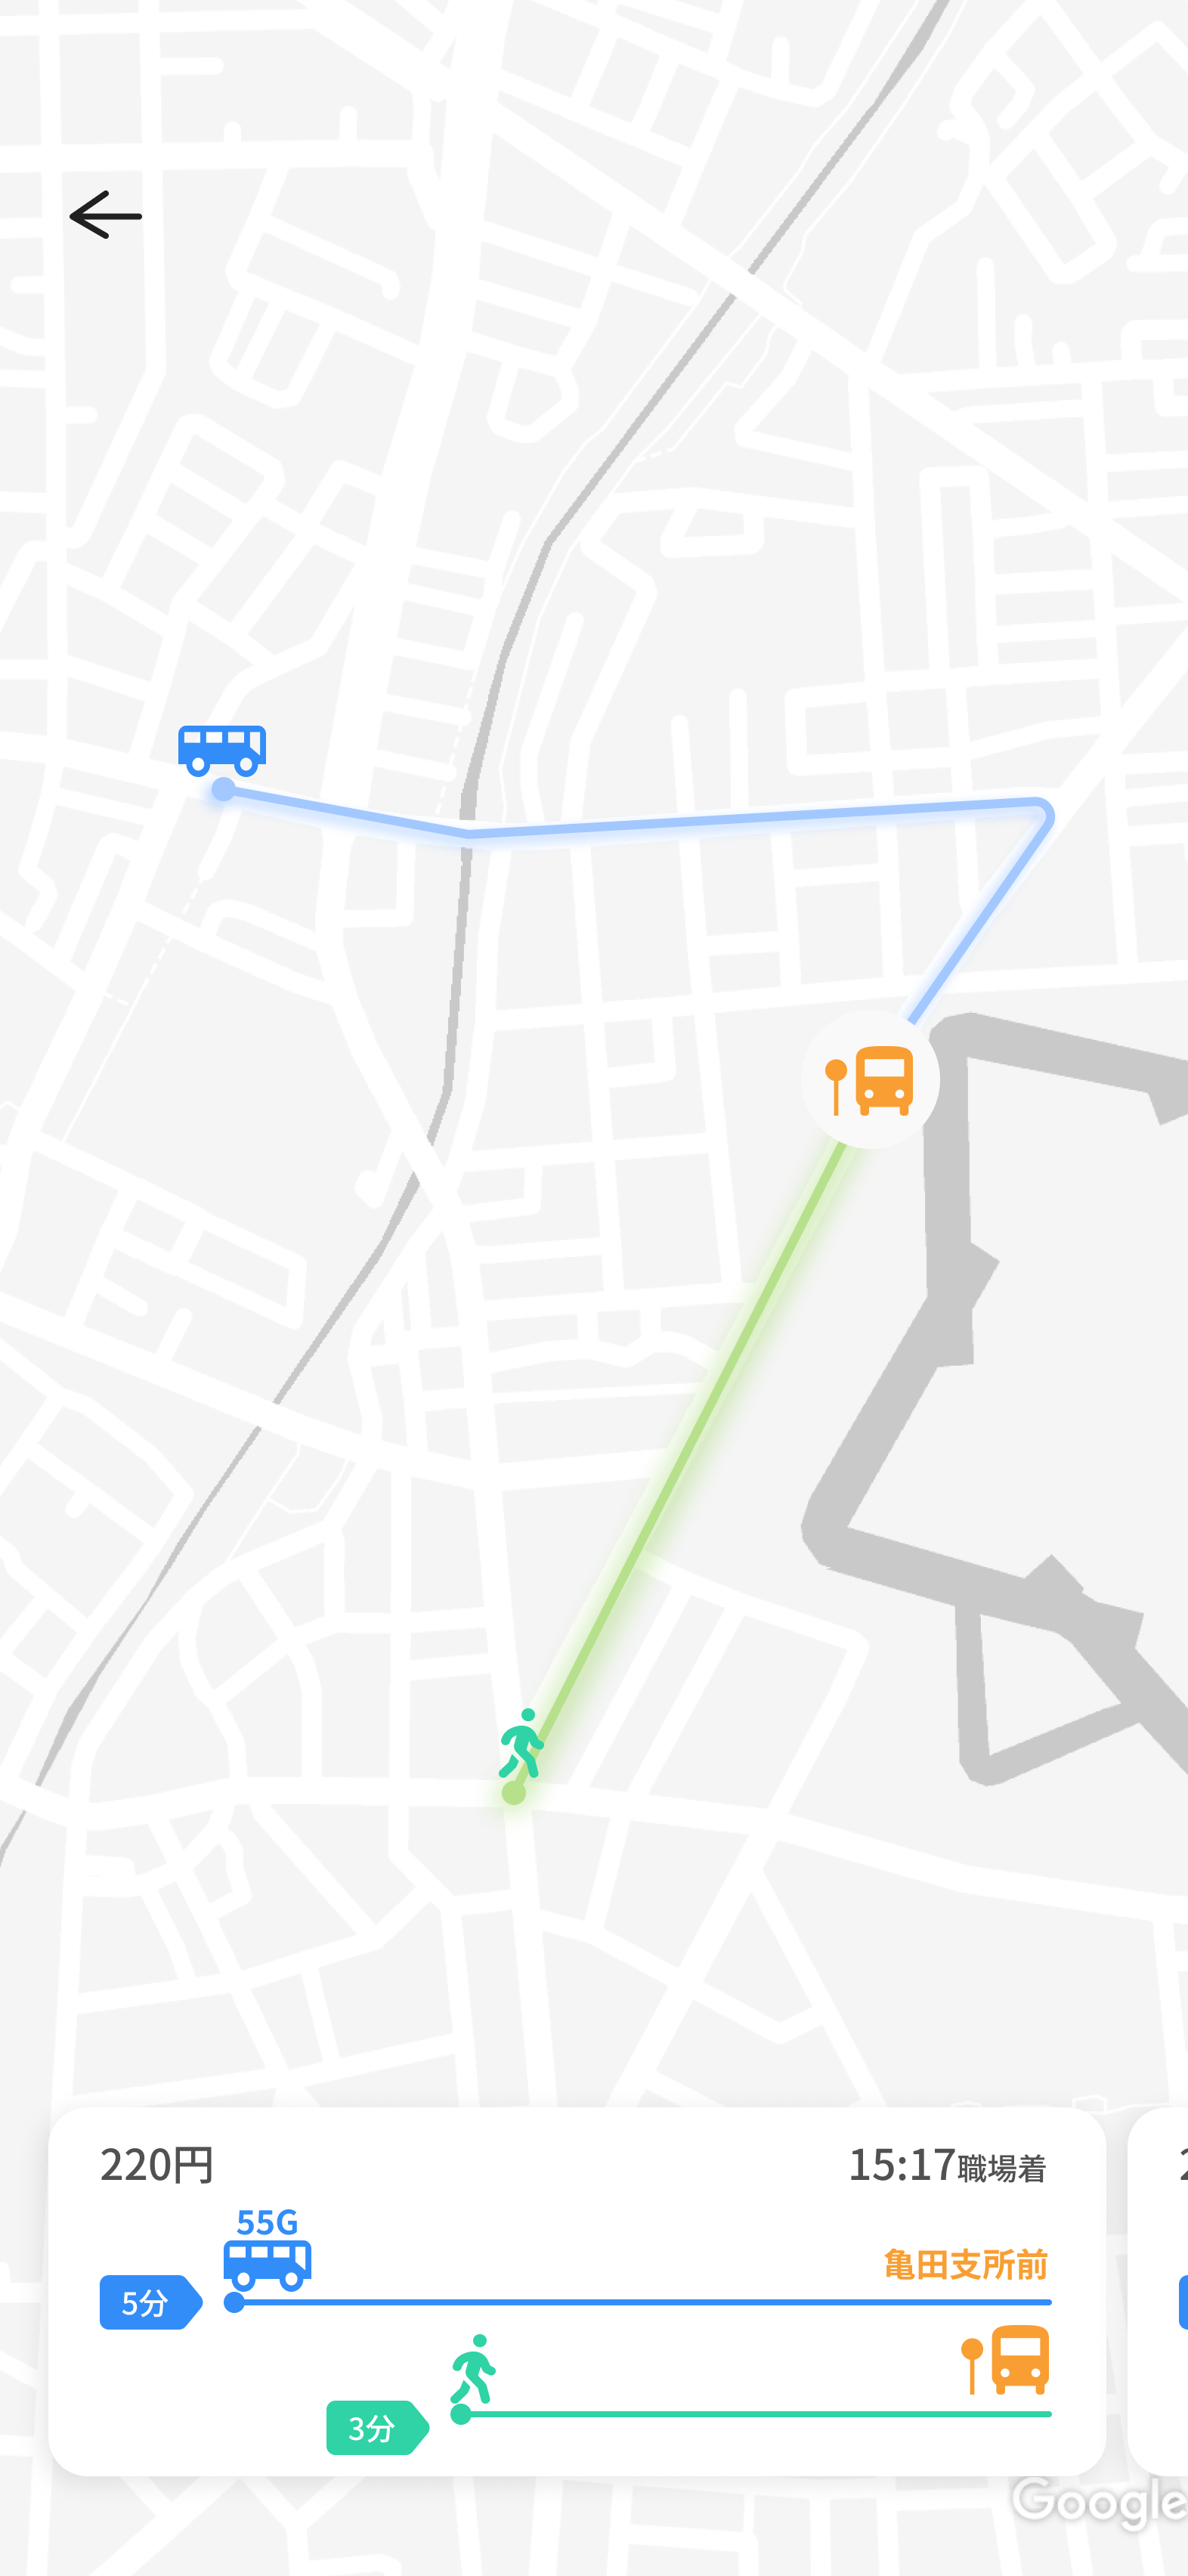
\includegraphics[width=6cm]{images/feature_routeview.png}
    \caption{バス位置情報閲覧機能}
    \label{fig:feature_routeview}
\end{figure}
\bunseki{下村蒔里萌}

\chapter{今後の活動}
今後の活動予定は,引き続きアプリ開発をすすめ8月中にアプリのバージョン1.0のリリースを目指す.そこで使用したユーザからのフィードバックをもとにアプリのデザイン,機能の改善を行っていく.また9月17日,18日にはUCDワークショップへの参加を予定している.前期では教員,プロジェクトメンバーからのフィードバックにより,機能,UIの改善を行ったため,今後はそれをもとに実際にアプリの開発を進めていく.またアプリへの認識の違いにより,思うようにアプリの具現化を行うことができなかったので,それも今後は共通認識を持てるように工夫し活動をしていく.
\bunseki{大津武琉}


\begin{appendix}

\chapter{使用技術・ツール・知識}
\section{フレームワーク}
\subsection{Flutter}
モバイルアプリのフレームワークとしてFlutter\footnote{https://flutter.dev/}を用いた.Android,iOSの両者にサービスを展開する上でKotlin,Swiftそれぞれでネイティブアプリを作成する事も検討したが,グループの規模とメンバーの技術力を考慮して,クロスプラットフォーム開発が可能であるFlutterを用いることに決定した.

\section{ツール}
\subsection{Discord}
本グループの主な連絡手段としてDiscord\footnote{https://discord.com/}を使用した.プロジェクトの連絡はもちろん,日常生活で起こったことなどをDiscordで共有することによりチームワークの向上を実現することができた.

\subsection{Notion}
本グループでは情報を管理するツールとしてNotion\footnote{https://www.notion.so/}を使用した.議事録,日報,週報,プロダクトバックログをそれぞれページにまとめることにより,情報を見やすくすることができた.今後も情報の管理ツールとして使用をしていく.

\subsection{GitHub}
GitHub\footnote{https://github.com/}とはソースコードのバージョン管理システムである.このツールを用いることでチームでのアプリ開発を効率的に行うことができる.本グループではフロントエンド,バックエンドでそれぞれリポジトリを作成し,アプリの開発を進めている.今後はより一層アプリの開発を進めることとなるため,GitHubを利用していく.
\pagebreak
\subsection{Figma}
Figma\footnote{https://www.figma.com/}とは,ホームページやアプリケーションなどのワイヤーフレームを作成できるツールである.中間発表スライドの作成,プロトタイプの作成,函館バス訪問の際に使用したスライドの作成に使用した.コンポーネントやレスポンシブを意識し,ワイヤーフレームを作成することで,今後の開発がスムーズになるようにした.

\subsection{Slack}
本プロジェクトの主な連絡手段としてSlack\footnote{https://slack.com/}を使用した.本グループでは主な連絡手段としてDiscordを利用していたが,プロジェクトではSlackを利用するとなったため使用した.細かくチャンネルを分けることで情報がどこにあるかをわかりやすくすることができた.また,メンションという機能を利用することにより教員,プロジェクトメンバー,TAとそれぞれに通知が行くようにすることで効率の良い意思疎通を行うことができた.

\subsection{Miro}
Miro\footnote{https://miro.com/}はオンラインでホワイトボードを利用できるツールである.ブレインストーミングなど,メンバーで一斉に意見を書くときに使用した.Miroを使用することにより,メンバーそれぞれの意見,考えを効率よく共有することができた.現在は同じような機能を持ったFigJamを利用している.

\subsection{FigJam}
FigJam\footnote{https://www.figma.com/}はオンラインでホワイトボードを利用できるツールである.Miroと同じようなツールだが本グループではFigmaを利用しており同じサービス元であるためFigJamへと移行した.

\subsection{Google Drive}
Google Drive\footnote{https://drive.google.com}とはGoogleが提供するオンラインストレージサービスである.これを用いることにより手軽にファイルの共有を行うことができる.また昨年度のファイル履歴を見返すこともでき,資料作り,プロジェクトの進め方の参考とした.
\pagebreak
\section{マネジメント}
\subsection{リスクマネジメント}
プロジェクトを行ううえでリスクは必ず存在する.リスクマネジメント\cite{risk}はそのリスクに対してどのように対策するのかを考える.まず初めにプロジェクトメンバーを3グループに分け,それぞれのチームでメンバーが持ち寄った起こりそうなリスクをまとめた.その後それぞれのリスクに対して,そのリスクが被る被害,発生確率,影響度,脅威,対策を考えた.脅威については発生確率,影響度を掛け合わせたものであり,脅威の値が大きいほど対策するべき優先度が高いものとなる.

\chapter{活用した講義}
\section{アジャイルワークショップ}
アジャイルコーチの永瀬氏に,本プロジェクトで用いるチーム開発の手法であるアジャイル開発について講義をしていただいた.まず,本ワークショップの前に事前知識を得るため,アジャイル開発についてのビデオを視聴した.その知識をもとに永瀬氏からアジャイル開発とはなにか,アジャイル開発で用いられるスクラムとはなにかを学んだ.また,最後に講義を受けているメンバーを5人ずつのチームにし,スクラムについてのクイズ大会を行った.これにより,楽しみながらスクラムについて学ぶことができ,スクラムについての共通認識を持つことができた.

\section{フィールドワーク講座}
本プロジェクトの担当教員でもある,南部美砂子准教授,元木環准教授に講義をしていただき,フィールドワークに関する基本的な考え方,ありがちな間違いをご教授いただいた.収束的なフィールドワークでは,思い込みや認識の狭さなどを超えられないため,フィールドワークには問題を探しにいくのではないこと,また,人々の行為や相互行為には必ず理由や動機が存在し,それらを理解することをフィールドワークの目的とすることを学んだ.

\end{appendix}

\begin{thebibliography}{3}
    \bibitem {scrum} 西村 直人, 永瀬 美穂, 吉羽 龍太郎. SCRUM BOOT CAMP THE BOOK スクラムチームではじめるアジャイル開発. 株式会社 翔泳社. 2020.
    \bibitem {scrummaster} Zuzana Sochova. SCRUM MASTER THE BOOK. 株式会社 翔泳社. 2020.
    \bibitem {risk} 株式会社インターリスク総研,リスクマネジメント入門. https://www.ms-ins.com/pdf/business/rm/rmguide.pdf (2023/07/12)
\end{thebibliography}

\end{document}
